\documentclass[]{IEEEtran}

\usepackage[utf8]{inputenc}
\usepackage{float, graphicx, booktabs, siunitx}
\usepackage{microtype, amsmath, minted, siunitx}

\usepackage{inconsolata}
\usepackage[italian]{babel}

\newcommand{\tool}[1]{\textsf{#1}}
\newcommand{\code}[1]{\mintinline{text}{#1}}

\title{Modellazione in VHDL di un cifrario basato su algoritmo XTEA}
\author{Massimiliano Incudini - VR433300}

\begin{document}
\maketitle

\begin{abstract}
    Il seguente documento documenta il lavoro svolto durante la seconda parte del modulo di laboratorio del corso Progettazione di Sistemi Embedded (aa 2018/2019). Il suo obiettivo è illustrare le scelte progettuali effettuate durante lo sviluppo del modulo XTEA nel linguaggio VHDL.
\end{abstract}
\section{Introduzione}

Il progetto consiste nello sviluppare un cifrario il cui funzionamento è basato sull'algoritmo eXtended TEA fornito insieme alla consegna.
\begin{enumerate}
    \item Il cifrario dovrà essere implementato come modulo VHDL, poi testato automaticamente tramite uno script \code{stimuli.do} per il software proprietario \textsf{\small Modelsim}.
    \item Il modulo deve essere importato in \textsf{\small Vivado}, simulato tramite un testbench e sintetizzato per la piattaforma \textsf{\small Xilinx PYNQ}.
    \item I sorgenti SystemC del cifrario dovranno essere sintetizzati tramite \textsf{\small Vivado HLS}, ed il risultato della sintesi confrontato con quello del modulo VHDL.
\end{enumerate}

\section{Architettura del modulo}

Il modulo cifratore presenta gli ingressi e le uscite visibili in Figura~\ref{fig:layout}.

\begin{figure}[h]
    \centering
    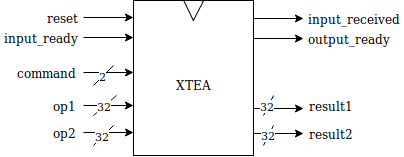
\includegraphics[width=0.4\textwidth]{vhdl_schemi/layout.png}
    \caption{Interfaccia del modulo VHDL}
    \label{fig:layout}
\end{figure}

In input abbiamo:
\begin{itemize}
    \item \code{clock} (1bit): segnale di sincronia;
    \item \code{reset} (1bit): quando alto resetta il modulo alle condizioni iniziali;
    \item \code{input_ready} (1bit): quando alto il modulo può leggere i valori sulle porte \code{command}, \code{op1} e \code{op2};
    \item \code{command} (2bit): operazione da eseguire, deve essere uno tra i valori \code{CONFIGURE_KEYS_0_1}, \code{CONFIGURE_KEYS_2_3}, \code{RUN_ENCRYPT}, \code{RUN_DECRYPT};
    \item \code{op1} (32bit): primo operando;
    \item \code{op2} (32bit): secondo operando.
\end{itemize}
In output abbiamo:
\begin{itemize}
    \item \code{input_received} (1bit): quando alto il modulo segnala di aver letto i valori in input;
    \item \code{output_ready} (1bit): quando alto il modulo segnala completato l'operazione ed è in grado di ricevere nuovi comandi;
    \item \code{result1}, \code{result2} (32bit ciascuno): prima e seconda parte del risultato.
\end{itemize}

Il modulo per poter criptare o decriptare ha bisogno in input di 6 parole a 32bit: quattro appartenenti alla chiave di cifratura, e due appartenenti al messaggio. Abbiamo quindi una prima fase di configurazione, nel quale impostiamo la chiave. Non occorre ripetere questa prima fase se non per cambiare la chiave o dopo un reset. Successivamente possiamo passare il messaggio, due word alla volta, al modulo per effettuare l'operazione richiesta. Questo meccanismo è schematizzato in Figura~\ref{fig:algo}.

\begin{figure}[ht]
    \centering
    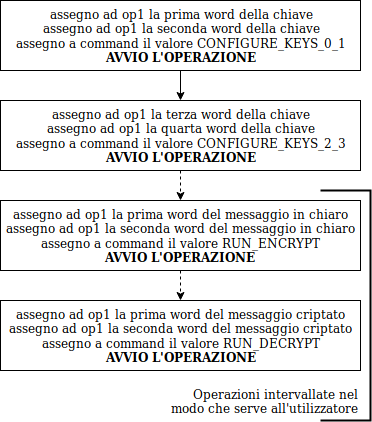
\includegraphics[width=0.36\textwidth]{vhdl_schemi/algo.png}
    \caption{Operazioni del modulo}
    \label{fig:algo}
\end{figure}

Ognuna delle operazioni segue un preciso protocollo illustrato in Figura~\ref{fig:handshake}. Per prima cosa l'utilizzatore scrive sulle porte dei dati e alza \code{input_ready}. Il modulo legge i dati ed abbassa \code{output_ready}. Il ciclo di clock successivo il modulo alza \code{input_received}. A questo punto l'utilizzatore abbassa \code{input_ready}. Una volta che il modulo ha completato l'operazione scrive sulle porte di output i risultati, alza \code{output_ready} ed abbassa \code{input_received}. 

\begin{figure}[ht]
    \centering
    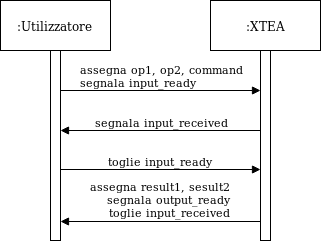
\includegraphics[width=0.36\textwidth]{vhdl_schemi/handshake.png}
    \caption{Protocollo di esecuzione di una qualsiasi operazione}
    \label{fig:handshake}
\end{figure}

\section{Implementazione}

Il modulo è implementato nel file \code{xtea.vhd}. La sua struttura è quella di una FSMD, e divisa in tre processi.
\begin{itemize}
    \item Il primo processo scandisce lo step di computazione, ha nella sua sensitivity list il \code{clock} e serve per aggiornare il segnale \code{current_state}. 
    \item Il secondo processo implementa la FSM, aggiorna i segnali di controllo tra cui \code{next_state}, \code{input_received} e \code{output_ready}, nonchè legge e immagazzina i dati in input. 
    \item Il terzo processo implementa il datapath, effettua i calcoli sui dati in input e scrive i dati in output. 
\end{itemize} 
Lo schema della E-FSM associata al modulo è visibile in Figura~\ref{fig:efsm}. Inoltre, le costanti rappresentanti i comandi del modulo sono presenti nel file \code{xtea_helper.vhd}.

\begin{figure}
    \centering
    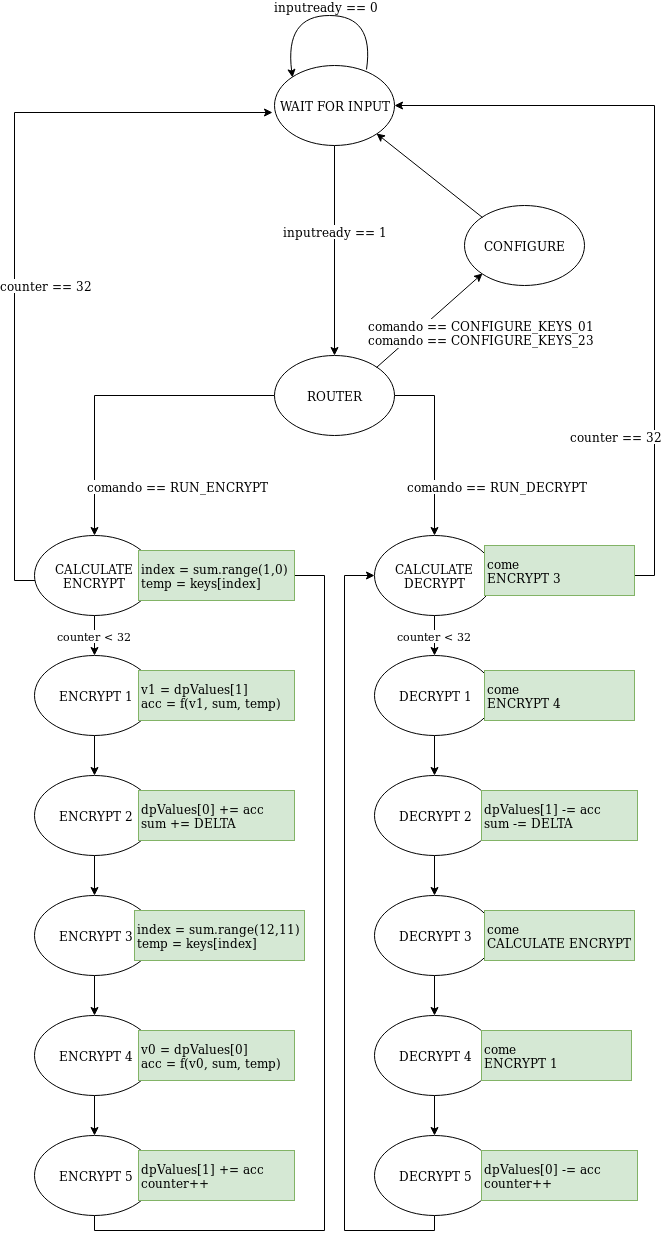
\includegraphics[width=0.48\textwidth]{vhdl_schemi/fsm.png}
    \caption{EFSM}
    \label{fig:efsm}
\end{figure}

\section{Simulazione con \textsf{Modelsim}}

\begin{figure*}[tb]
    \centering
    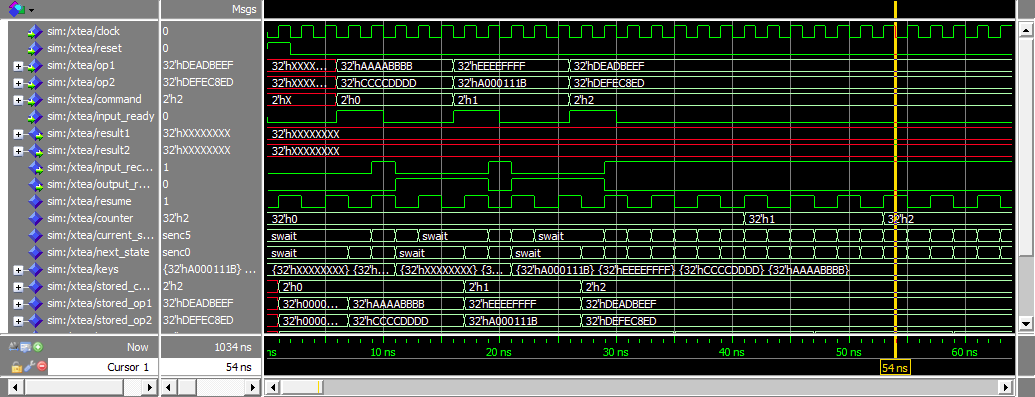
\includegraphics[width=\textwidth]{vhdl_schemi/modelsim.png}
    \caption{Porzione della simulazione. La fase di reset parte a 0ns. Le fasi di configurazione della prima e della seconda parte delle chiavi partono a 6ns e 16ns. La fase di criptazione del messaggio parte a 21ns.}
    \label{fig:modelsim}
\end{figure*}

Per poter simulare il progetto col software \textsf{Mentor Modelsim} creiamo un nuovo progetto all'interno del quale importiamo i file \code{xtea.vhd} e \code{xtea_helper.vhd}. Nella console digitiamo i comandi:
\begin{minted}[fontsize=\footnotesize]{tcl}
# Compilazione del file e visualizzazione report
vcom -reportprogress 300 -work work C:/percorso/xtea.vhd
# Apertura software di simulazione
vsim [-wlf output_waveform_file.wlf] work.xtea
do stimuli.do
# Chiusura simulazione
quit -sim
\end{minted}

Segue una parte del file \code{stimuli.do} che automatizza in parte il setup della simulazione. Il comando \code{force <porta> <valore> <tempo di assegnazione> ns} assegna al tempo voluto il valore alla porta. Così facendo possiamo comandare in modo molto immediato il nostro modulo. L'alternativa a questo sarebbe scrivere un file VHDL di testbench. 

Il metodo qui utilizzato ha una limitazione. Quando eseguiamo un'operazione, mettiamo \code{input_ready} alto, e poi lo abbassiamo quando viene segnalato \code{input_received}. Non avendo un'istruzione del tipo ``esegui fino a che \code{input_received = 1}" decidiamo di aspettare due cicli di clock, dopo i quali sappiamo dall'implementazione che tale segnale viene messo alto. Se però l'implementazione cambiasse allora questo sistema non funzionerebbe più.

Per questo nelle sezioni successive utilizziamo un modulo testbench, che permette una simulazione più ``robusta". 

\AtBeginEnvironment{minted}{%
  \renewcommand{\fcolorbox}[4][]{#4}}
\begin{minted}[fontsize=\footnotesize]{tcl}
# fai ripartire la simulazione (se non lo fai, 
# continua dal punto nel quale si era fermato)
restart -f 

# tolgo e ri-aggiungo i segnali del modulo alla schermata
delete wave *
add wave *

# RESET DEL MODULO
# il clock parte con 0, resta basso 1ns, viene alzato, 
# resta alto 1ns, e ripeto il processo ogni 2ns
force clock 0 0 ns, 1 1 ns -repeat 2
force reset 1 0 ns, 0 2 ns
force input_ready 0 0 ns
run 10ns

# CONFIGURAZIONE PRIMA PARTE DELLE CHIAVI
# i segnali che dico partire da 0ns non ripartono davvero
# dell'inizio ma dal punto in cui si era fermata la sim.
force op1 16#AAAABBBB 0 ns
force op2 16#CCCCDDDD 0 ns
force command 2#00    0 ns
force input_ready 1   0 ns
run 4 ns
force input_ready 0   
run 6 ns
\end{minted}

Il software permette di salvare le forme d'onda nel formato proprietario \code{wlf}. Una porzione di questa è visibile in Figura~\ref{fig:modelsim}. All'occorrenza, questo può essere convertito nel formato aperto \code{vcd} con il tool \code{wlf2vcd}. Il risultato può essere visto con il software \textsf{Gtkwave}. 



\section{Sintesi in Vivado}

I sorgenti utilizzati all'interno di \tool{Modelsim} vengono importati in \tool{Xilinx Vivado}. 

Il modulo viene testato ora attraverso un modulo testbench \code{xtea_tb.vhd}. Questo mima il comportamento del file di stimoli ma in modo più agevole, poichè il linguaggio VHDL permette istruzioni \mintinline{vhdl}{wait port'event and port = '1'} che permettono di aspettare indefinitamente l'evento su una porta prima di proseguire con il resto del codice, anzichè obbligarci a fare i calcoli della temporizzazione a mano. 

Una volta che abbiamo appurato il corretto funzionamento del modulo, procediamo con la sintesi. Il modulo viene sintetizzato per la piattaforma PYNQ con codice \code{xc7z020clg400-1}. Il modulo risulta sintetizzabile, e le risorse utilizzate risultano quelle di Tabella~\ref{tab:utilizzo}.

\begin{table}[htbp]
    \centering
    \begin{tabular}{l S[table-format=3.0] S[table-format=3.0] S[table-format=6.0] S[table-format=0.2] }
        \toprule
        {Site Type}        	    & {Used}     & {Fixed} 	 & {Available} 	  & {Util (\%)} \\ \midrule
 Slice LUTs*             	    & 486	     &     0	 &    53200	      & 0.91 \\
 \quad LUT as Logic          	& 486	     &     0	 &    53200	      & 0.91 \\
 \quad LUT as Memory         	& 0	         &     0	 &    17400	      & 0.00 \\
 Slice Registers         	    & 441	     &     0	 &    106400	  & 0.41 \\
 \quad Register as Flip Flop 	& 15	     &     0	 &    106400	  & 0.01 \\
 \quad Register as Latch     	& 426	     &     0	 &    106400	  & 0.40 \\
 F7 Muxes                	    & 0	         &     0	 &    26600	      & 0.00 \\
 F8 Muxes                	    & 0	         &     0	 &    13300	      & 0.00 \\\bottomrule
    \end{tabular}
    \caption{Utilizzo delle componenti di \code{xtea}}
    \label{tab:utilizzo}
\end{table}

L'implementazione su FPGA risulta invece un problema col design attuale. Infatti la scheda seleziona permette di poter solamente 125 porte di input/output mentre per il nostro modello ne servono 135. Se volessimo utilizzare il modulo come sistema standalone sulla scheda, dobbiamo trovare il modo di ridurre il numero di IO. Una soluzione semplice è implementare un componente wrapper di \code{xtea}, con porte dati più piccole, che passano i valori al nostro modulo in più cicli di clock (\code{input_ready} viene messo a 1 solo quando il valore è stato salvato completamente).

Viene fatta l'implementazione di questo componente all'interno del file \code{xtea_s2p.vhd}. L'implementazione avviene correttamente, e le porte di IO usate sono 38.

In ogni caso, si presuppone che il cifratore sia inserito all'interno di un sistema embedded più ampio, quindi il problema del numero di porte in realtà è meno grave di quanto ipotizzato inizialmente.


\section{Sintesi ad alto livello con Vivado HLS}

Proviamo ad importare il file di specifiche del modulo all'interno di \textsf{Vivado HLS}. L'unico file fornito viene diviso in un sorgente ed in un testbench (quest'ultimo contiene la sola funzione \code{main}). 

Per testare la correttezza delle specifiche avviamo la simulazione del codice C. Il risultato è corretto e ne segue il log (stampa del logo omessa):
\begin{minted}[fontsize=\footnotesize]{text}
INFO: [SIM 2] *************** CSIM start ***************
INFO: [SIM 4] CSIM will launch GCC as the compiler.
   Compiling ../../xtea_tb.cpp in debug mode
   Compiling ../../xtea.cpp in debug mode
   Generating csim.exe
First invocation: 
   - the encryption of 12345678 and 9abcdeff 
   - with key 6a1d78c88c86d67f2a65bfbeb4bd6e46 
   is: 99bbb92b, 3ebd1644 
Second invocation: 
   - the decryption of 99bbb92b and 3ebd1644 
   - with key 6a1d78c88c86d67f2a65bfbeb4bd6e46 
   is: 12345678, 9abcdeff 
Done!!
INFO: [SIM 1] CSim done with 0 errors.
INFO: [SIM 3] *************** CSIM finish ***************
\end{minted}

Infine avviamo la sintesi. In output abbiamo un file \code{xtea.vhd}. Questo viene importato in \textsf{Vivado} e sintetizzato. La sintesi ha esito positivo. L'implementazione ha esito negativo sempre a causa del numero di IO. 

\begin{table}[htbp]
    \centering
    \begin{tabular}{l S[table-format=3.0] S[table-format=3.0] }
        \toprule
        {Site Type}        	    & {VHDL RTL} & {Specifiche C++} \\ \midrule
 Slice LUTs              	    & 486	     &    696	 \\
 \quad LUT as Logic          	& 486	     &    696	 \\
 \quad LUT as Memory         	& 0	         &    0      \\
 Slice Registers         	    & 441	     &    606    \\
 \quad Register as Flip Flop 	& 15	     &    606    \\
 \quad Register as Latch     	& 426	     &    0      \\
 F7 Muxes                	    & 0	         &    0	     \\
 F8 Muxes                	    & 0	         &    0	     \\ \bottomrule
    \end{tabular}
    \caption{Confronto}
    \label{tab:confronto}
\end{table}

\section{Conclusioni}

La Tabella~\ref{tab:confronto} confronta l'utilizzo di componenti delle varie versioni del modulo.

Vediamo come la versione VHDL occupa circa il 15\% delle risorse (porte logiche, memoria) rispetto alla versione sintetizzata a partire dalle specifiche. La perdita di spazio è in realtà irrisoria rispetto al tempo perso per implementare il VHDL, quindi è abbastanza ovvio che questa prima versione è da preferirsi. 

Infine notiamo come la versione VHDL utilizzi un certo numero di latch invece che flip-flops, sintomo esiste un processo in cui uno o più segnali vengono scritti in alcuni branch mentre in altri no. Questo difetto è prodotto da una svista del programmatore. Nella versione sintetizzata questi problemi non compaiono.

\end{document}